\section{features}
A fully interactive whitted-style raytracer with run time scene loading.

\subsection{Run time scene loader}
    \begin{enumerate}
    \item Json scene loader
        \begin{enumerate}
        \item Spheres, planes
        \item Triangle meshes - loaded from file, and transformed into the world (translate, rotate, scale)
        \item Point lights
        \item camera
        \end{enumerate}
    \item \verb|.obj| file loader (tinyojb)
    \item \verb|.mtl| material file loader (tinyobj)
    \end{enumerate}

\subsection{Materials}
    \begin{enumerate}
    \item diffuse lighting with hard shadows
    \item reflections
    \item transparency with refraction indices
    \item specular highlights
    \item diffuse, reflective and specular values are defined by a 3-value color to match the .mtl file format
    \end{enumerate}

\subsection{Camera}
    \begin{enumerate}
    \item resizable windows
    \item zoom (mousewheel)
    \item pitch, yaw and translate
    \end{enumerate}

\subsection{Lights}
    \begin{enumerate}
    \item multi-color lighting
    \item point lights
    \item spot lights - linear and log falloff models
    \end{enumerate}

\subsection{Other}
    \begin{enumerate}
    \item multi-platform with CMake (linux, mac and windows)
    \item multi-threaded with OpenMP (got around 5x speedup on linux, which is what is expected for 4 cores with HT)
    \end{enumerate}

\section{Building}

The source is built using the standard CMake envirnonment.

For example, on unix systems this command will do a release build -

\verb|cmake -DCMAKE_BUILD_TYPE=Release .|
\verb|make|

A similar command should work on Visual Studio, although the \verb|CMAKE_BUILD_TYPE| is not required - this is set in the Visual Studio gui.

On Windows, SDL2.dll must be available somewhere on the path or in the same dir as the binary. 

Boost is required for the test tree, but not the main system.

\section{Running}

There is a collection of test scenes, objects and materials in the data directory. To avoid fighting with relative paths, it works best to cd to this directory before running the system. For example, on windows, assuming the binary is in the Release directory under the root source tree - 

\verb|cd <source_root>\data|
\verb|..\Release\ray.exe col-lights.scene|

\section{Input Commands}
    \begin{enumerate}
    \item WASD - move around the world
    \item mouse movement - rotate camera (yaw/pitch)
    \item mouse wheel - zoom in/out
    \item R - reset camera view to default (possibly set from scene file)
    \item ESC - quit
    \item 0 - view ray-traced image (default)
    \item 1 - visualise per-line render time
    \item 2 - visualise surface normals
    \end{enumerate}

\section{External Packages}
The following external packages were used 
\begin{enumerate}
    \item tiny object loader --- \url{https://syoyo.github.io/tinyobjloader/}
    \item glm --- \url{https://glm.g-truc.net/0.9.8/index.html}
    \item JSON for Modern C++ --- \url{https://github.com/nlohmann/json}
    \item SDL2d
    \item boost (test tree only)
    \item CMake
\end{enumerate}

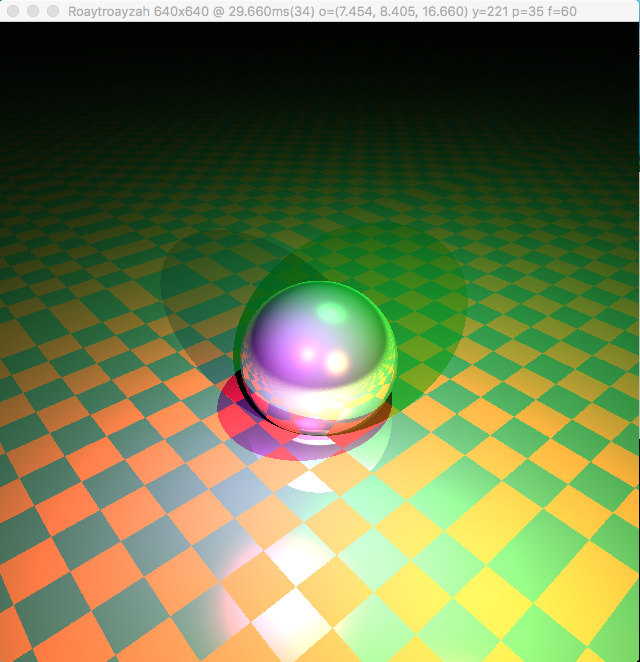
\includegraphics[width=0.5\textwidth]{img/colPointLights1sphere}
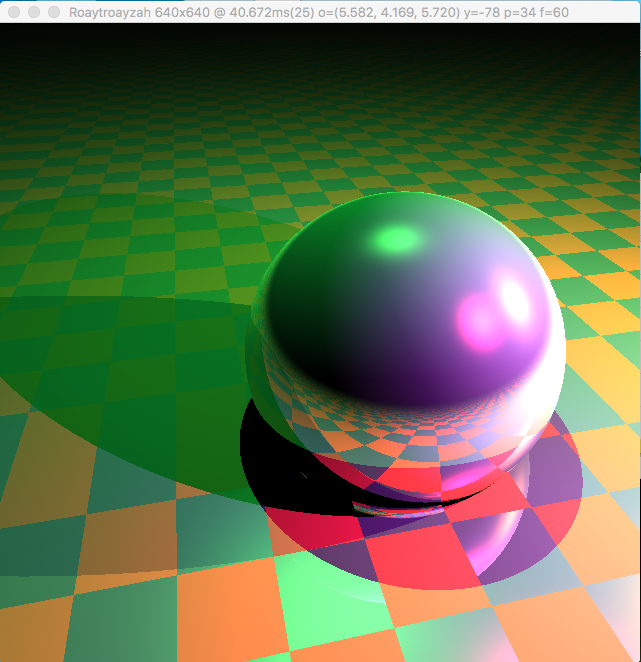
\includegraphics[width=0.5\textwidth]{img/colPointlights1sphere_close}
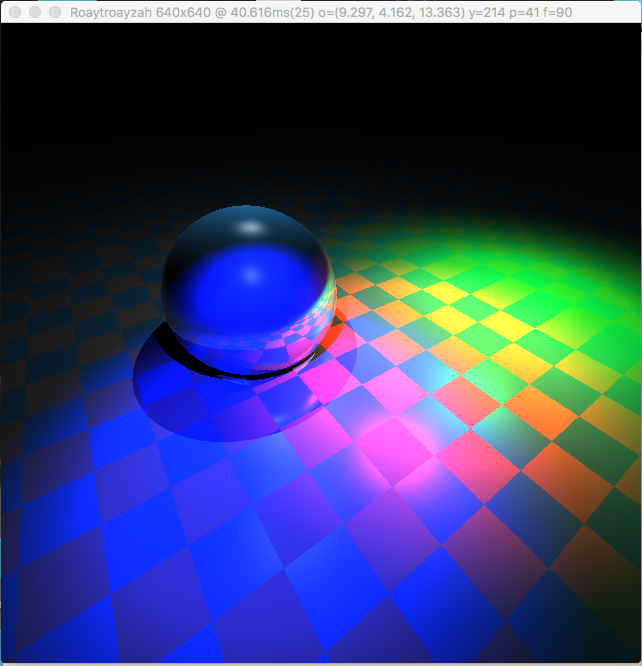
\includegraphics[width=0.5\textwidth]{img/colSpotlights1sphere}
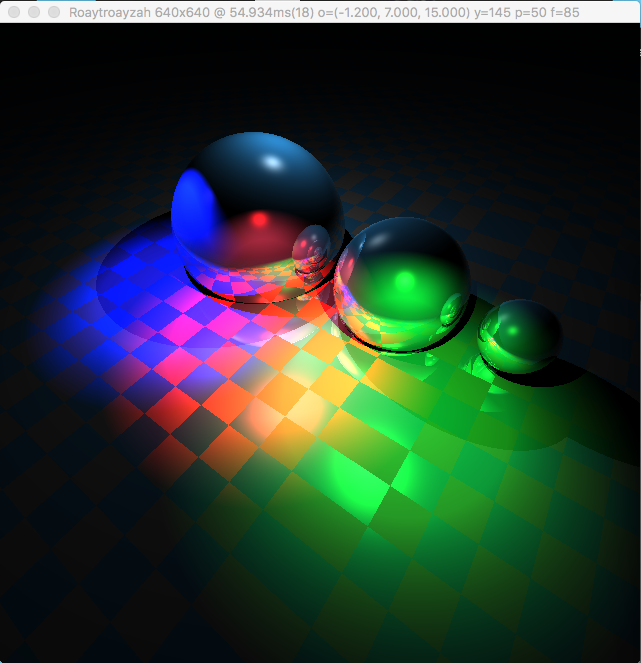
\includegraphics[width=0.5\textwidth]{img/colSpotlights3spheres}
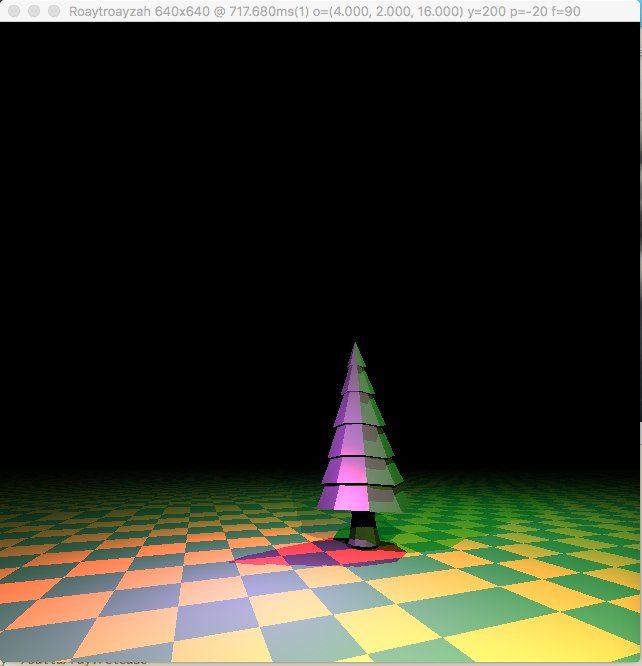
\includegraphics[width=0.5\textwidth]{img/colourLitTree}
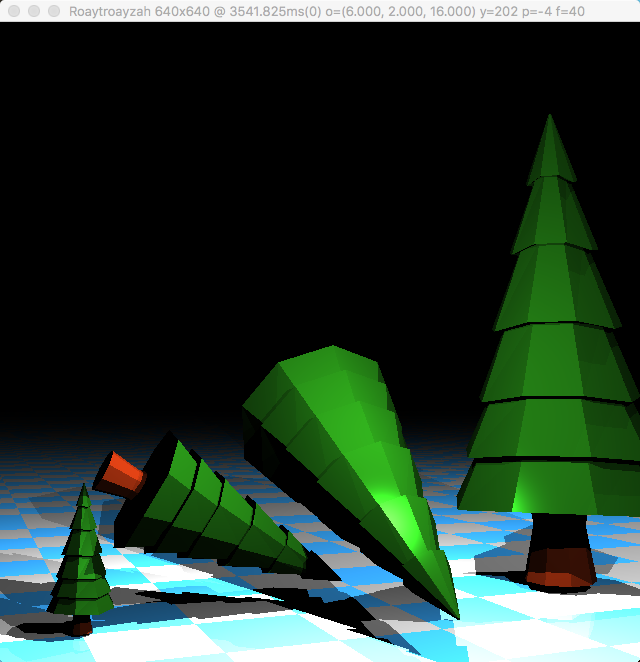
\includegraphics[width=0.5\textwidth]{img/fallingTrees}
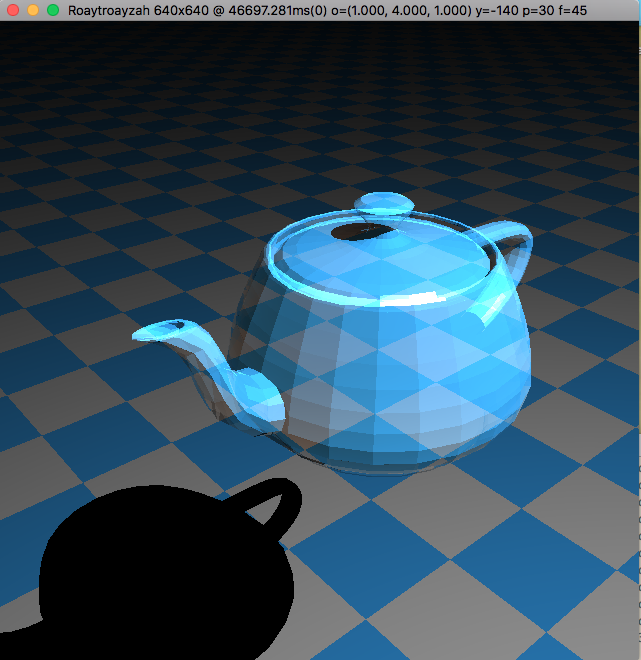
\includegraphics[width=0.5\textwidth]{img/ghostTeapot}
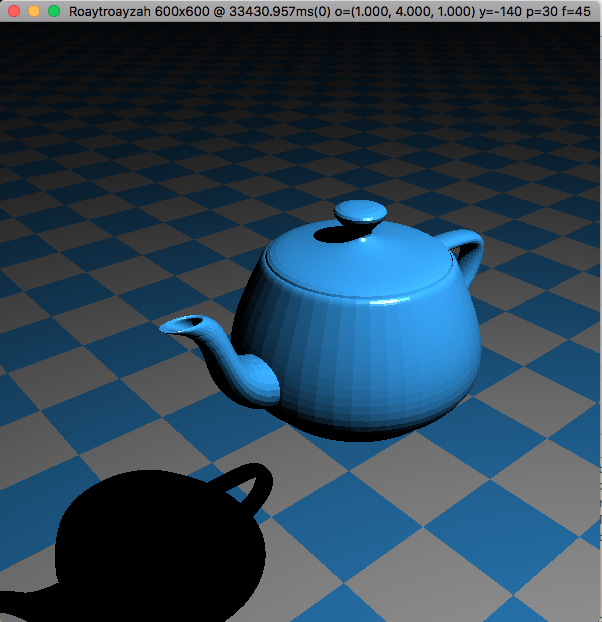
\includegraphics[width=0.5\textwidth]{img/hiresTeapot}
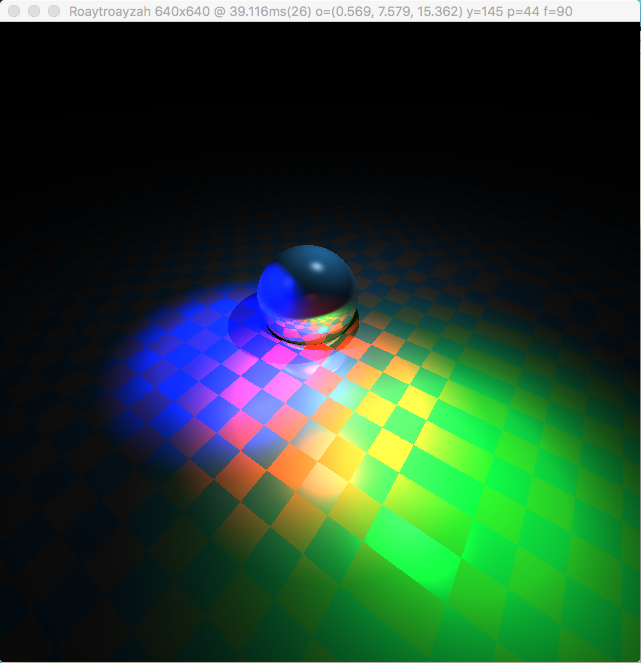
\includegraphics[width=0.5\textwidth]{img/niceSphere}
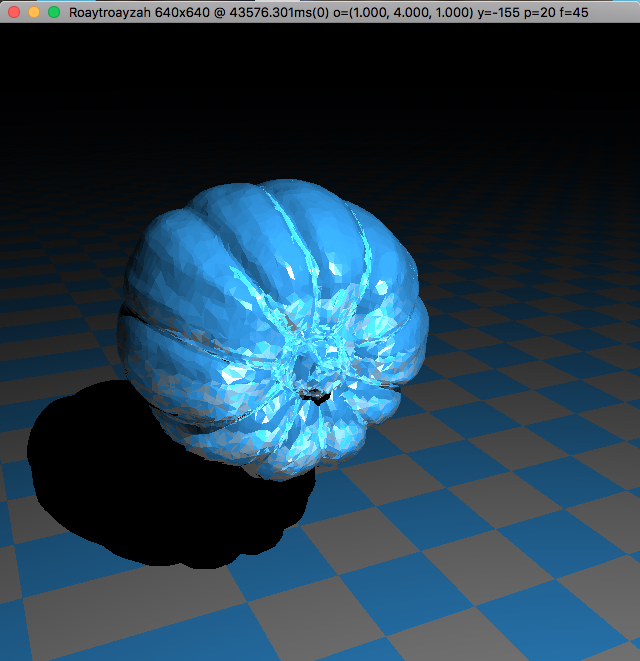
\includegraphics[width=0.5\textwidth]{img/pumpkin}
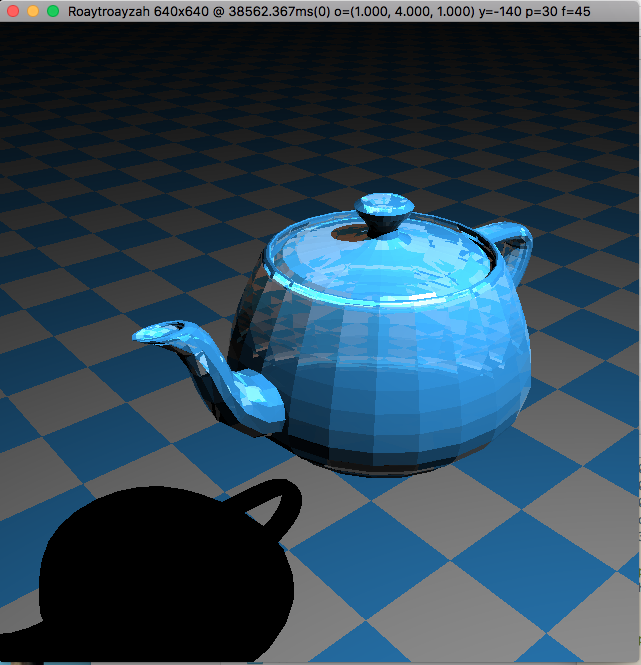
\includegraphics[width=0.5\textwidth]{img/refractingTeapot}
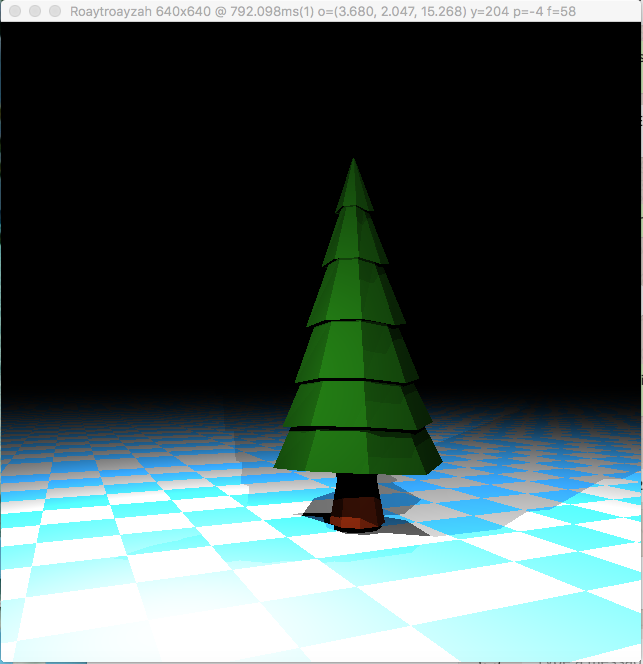
\includegraphics[width=0.5\textwidth]{img/simpleTree}
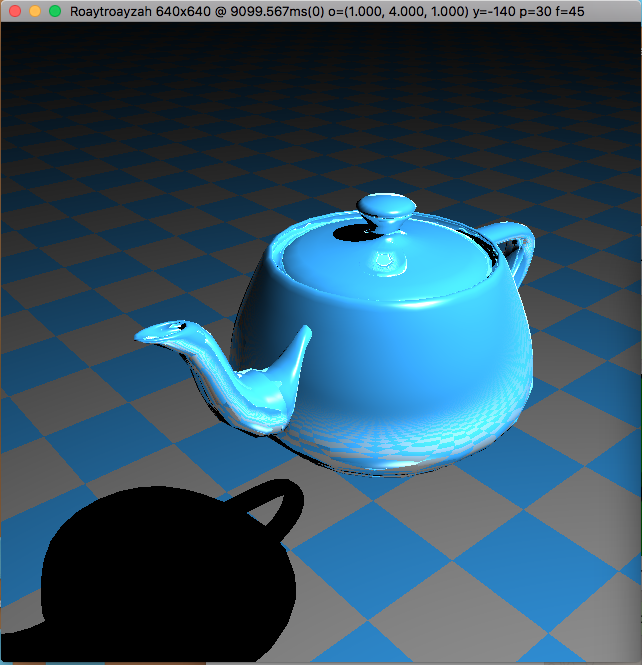
\includegraphics[width=0.5\textwidth]{img/smoothTeapot1}
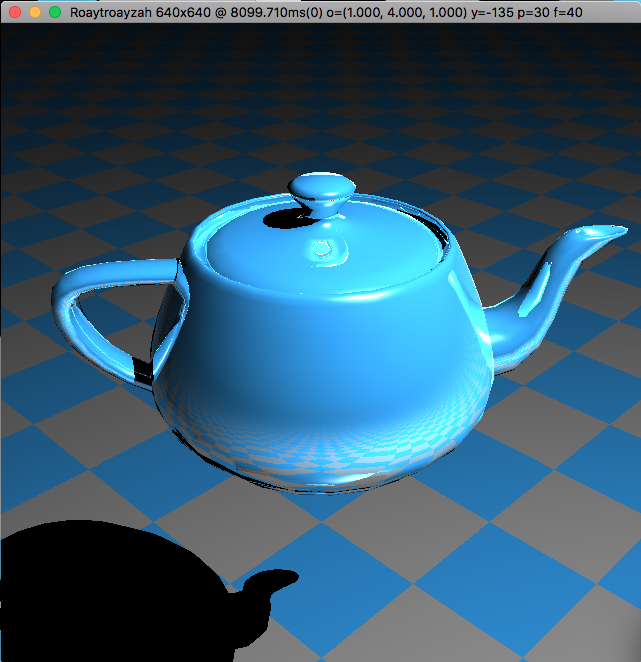
\includegraphics[width=0.5\textwidth]{img/smoothTeapot2}
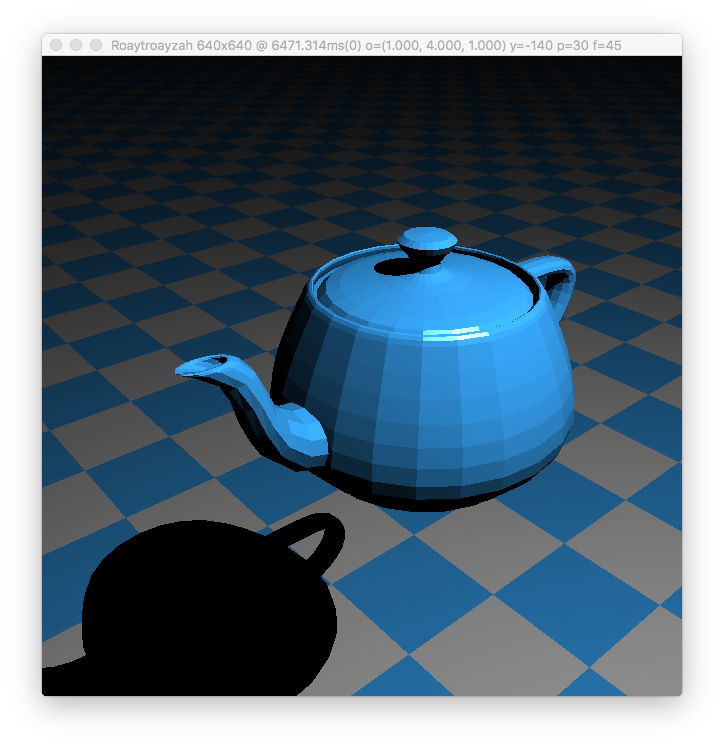
\includegraphics[width=0.5\textwidth]{img/solidTeapot}
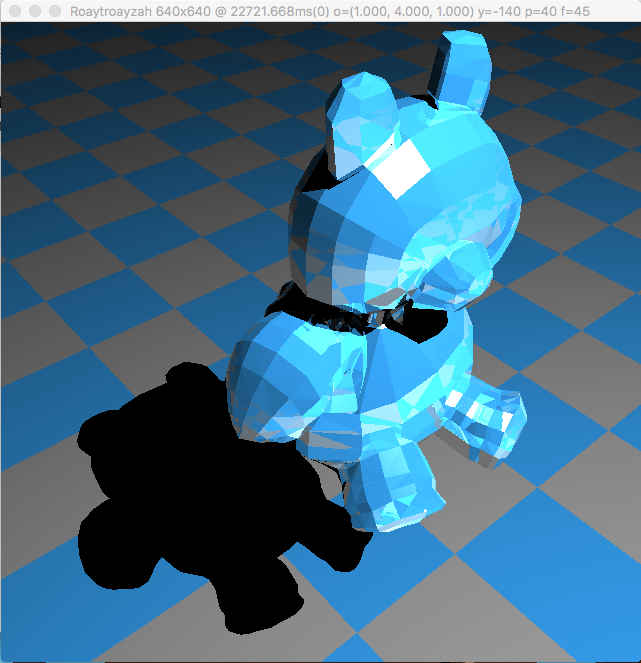
\includegraphics[width=0.5\textwidth]{img/teddy}
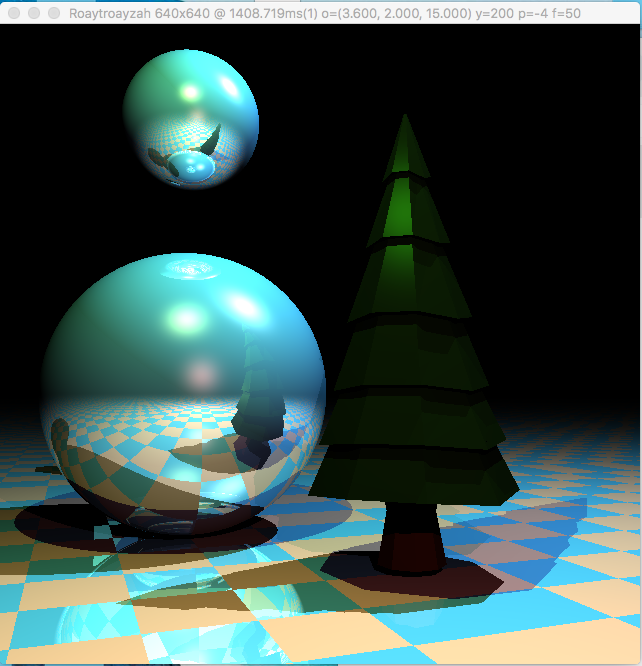
\includegraphics[width=0.5\textwidth]{img/treeSpheres}
